\section{Technical Approach and Research Thrusts}
\label{sec:approach}
\label{sec:thrusts}

\sysname creates a digital twin of an infrastructure, performs security tests
on the twin, and uses the results to improve the security posture of the
original. Three challenges shape the design. First, the configuration of the
original must be captured continuously, as complex infrastructures are in
constant evolution. Second, most large infrastructures cannot be fully
replicated, and the twin must be smaller in scale but still representative. Third, as the infrastructure evolves, the twin has to evolve
as well, or the results will describe a system that no longer exists.

\begin{figure}[!htbp]
\centering
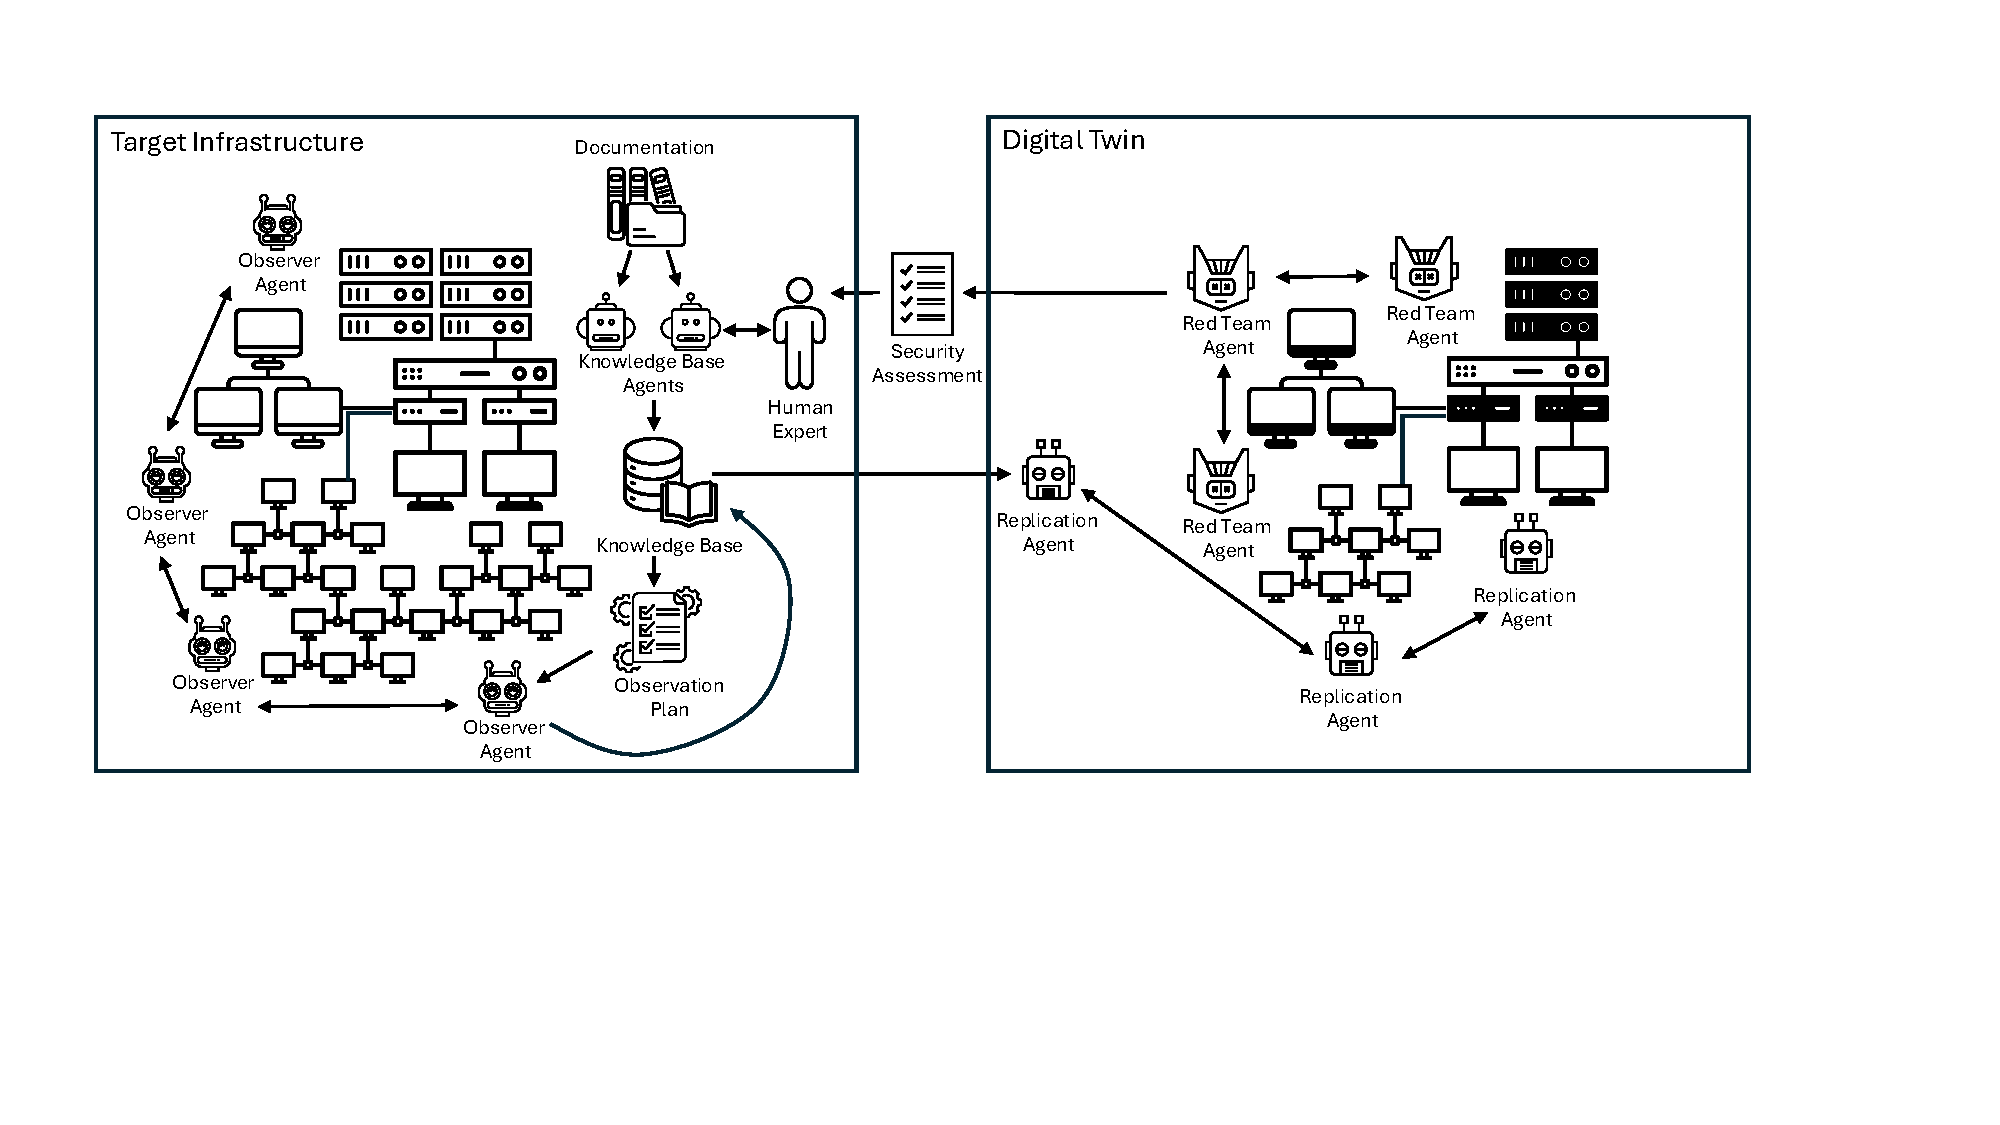
\includegraphics[width=\linewidth]{figures/redtwin_architecture.pdf}
\caption{Overview of the \sysname framework. Knowledge Base Agents combine
documentation with human expertise to build a Knowledge Base, driving an
Observation Plan that deploys Observer Agents, which collect dynamic
information without disrupting operations and feed it back. Replication
Agents construct a digital twin from the Knowledge Base, and Red Team Agents
continuously assess that twin, producing findings that are verified and
remediated on the target infrastructure.}
\label{fig:overview}
\end{figure}

\sysname addresses these challenges by leveraging four cooperating teams of
agents, summarized in Figure~\ref{fig:overview} and developed in the thrusts
below. The Knowledge Base Agents build and maintain the model of the target,
the Observer Agents enrich that model by watching the running system without
ever touching it, the Replication Agents construct the twin, and the Red Team
Agents attack the twin and report their findings to a human analyst. When a
finding is a false positive, or an artifact of an imprecise replication, the information flows back to the Knowledge Base and Observer Agents, so each
analysis cycle also improves the fidelity of the twin. In the health-care deployment of
Section~\ref{sec:intro}, this loop is what turns an undocumented
administrative endpoint, a permissive \texttt{proxy\_pass} rule, and a
deserialization flaw in a broker client library into a single reported chain
from a device gateway to the patient database.

\subsection{Thrust 1: Capturing Open-Source Infrastructure Configurations}
\label{sec:thrust1}

\paragraph{Knowledge base design.}
Structured data will be used to represent the network topology and the roles
of the various components. For this layer, we will use a graph database, such
as Neo4j~\cite{neo4j}, whose model is a natural fit for the questions that
\sysname must answer, such as which hosts can reach a given service, which
services share a credential store, and which paths connect an externally
exposed component to a sensitive asset, while a vector store, such as
Qdrant~\cite{qdrant} or Weaviate~\cite{weaviate}, will hold the
natural-language documentation. A research challenge in this
step is the design of a schema expressive enough to capture the
security-relevant structure of an arbitrary deployment, yet constrained
enough to support the queries and invariants used downstream. We will model
hosts, containers, services, network segments, credentials, data stores, and
trust relationships as typed nodes and edges, and we will attach to each of
them the \emph{provenance} of the information together with a
\emph{confidence} level. Both are essential, because the same fact may be
asserted by a configuration manual and contradicted by a runtime observation.
Version information must be fine enough to map a deployed component to the
package, release, and build options that determine its vulnerabilities, since the component name alone does not identify a vulnerability set, whereas
the version, the module set, and the directive configuration do.

\paragraph{Observation techniques.}
The Observer Agents monitor the system statically, through documentation,
code, configuration files, and infrastructure-as-code artifacts, and
dynamically, through the runtime observation of network and host activities.
Examples of these techniques are passive network analysis at key north-south
and east-west points, the interpretation of logs into a shared ontology by
means of LLMs, API monitoring through facilities such as eBPF or service
meshes like Istio~\cite{istio}, configuration monitoring through managers
such as Ansible~\cite{ansible} or Puppet~\cite{puppet}, and the ingestion of
alerts from IDS/IPS, EDR, or SIEM tools. In addition, we plan to extend our
previous work on service security dependency analysis~\cite{achilles}. That
research demonstrated that by observing the dynamic behavior of services it
is possible to derive their security properties and dependencies. Accurately modeling these dependencies is essential: any dependency missed
during capture is absent from the twin and therefore never exercised by the
analysis.

\paragraph{Safe active discovery: extending ZMap.}
Passive observation cannot resolve every question, because whether a service
is reachable from a given segment, and what version it runs, is often
answerable only by sending a packet. The stateless design of ZMap~\cite{zmap} makes it
the right foundation for this task, but its assumption that the marginal
effect of a probe is negligible does not hold inside a hospital or a plant.
We therefore plan to develop, and contribute upstream, four extensions:
\emph{impact-budgeted scheduling}, that imposes per-target budgets on probe
rate and concurrency derived from what the knowledge base records each host
to be, with hard interlocks that abort a sweep when the observed latency or
error rates degrade; \emph{knowledge-graph-native output}, that emits typed assertions with provenance and confidence, so discovery feeds
the schema directly; \emph{richer safe fingerprinting}, that extends the
ZGrab~\cite{zgrab} handshakes to recover the version and module detail needed
to map a service to an upstream package; and \emph{incremental re-scan},
that prioritizes re-probing where confidence has decayed. These extensions
address the reason why many operators decline to scan their own networks, and
they are a concrete Track~3 improvement to a widely used product.

\paragraph{Observation planning and coverage.}
We will formulate the synthesis of the observation plan as a constrained
optimization problem. Each candidate vantage point offers a certain amount of
information gain, at a cost expressed in terms of the load on the production
system, the intrusiveness of the deployment, and the consumption of scarce
resources such as LLM queries, and the plan maximizes the coverage of the
components most relevant to the security model while respecting hard
constraints, for example, never deploying an agent on a host that carries a
latency-sensitive clinical workload. Because observation is deliberately
non-aggressive, the resulting model is necessarily incomplete. We will therefore develop a
\emph{model coverage} metric that estimates what fraction of the infrastructure the capture has
resolved, using saturation analysis over observation time, cross-validation
among documentation, infrastructure-as-code, and runtime observation, and, on
the reference networks, direct measurement against withheld ground truth.
Coverage is reported alongside every finding, and it bounds every claim
\sysname makes about production.

\paragraph{Supply chain and the human loop.}
In addition, we will incorporate SBOMs and package manifests into the capture process, so the
knowledge base records not just what is running, but also where each
component came from. This addresses the socio-technical risks
described in Section~\ref{sec:landscape}, and it feeds the remediation loop
of Thrust~3. Note that, while the process is presented here as a sequence,
the agents will actually work continuously: new documentation triggers new
observation plans, and observations inconsistent with the documentation are
presented to the administrator for disambiguation. We envision this
as an agent-human collaboration, because deploying observer agents modifies
the infrastructure and must be vetted, but as the agents become more
knowledgeable, we expect that the level of interaction will diminish, and
Section~\ref{sec:evaluation} measures whether it does.

\subsection{Thrust 2: Replicating Computing Infrastructures}
\label{sec:thrust2}

The key problem in this thrust is how to build digital twins that are
scale-reduced and yet still representative of the original. We organize the
approach around three insights, and we then make faithfulness quantitative.

\paragraph{Insight 1: infrastructures replicate for load.}
If 200 file servers share the same operating-system image, package versions,
and firewall rules, they can be considered equivalent from a security
modeling perspective, and a single instance can stand for all of them. This reduces the veracity of the twin, because attacks that exploit resource
bottlenecks will not transfer. The abstraction is therefore a trade-off
between faithful replication and the minimization of resource usage, and the
fidelity measure defined below reports where a given twin sits on it. We will formalize this idea as an equivalence relation over the
components of the infrastructure. Two components are placed in the same class
when they agree on the attributes that determine their security behavior,
such as the software image and version, the set of open ports and exposed
services, the applicable firewall and access rules, the trust relationships
in which they participate, and their position in the network topology. The
twin then instantiates a single representative per class, together with a
\emph{multiplicity annotation}. A central research question is which
attributes must be included to preserve a given class of attacks, and we will
study it empirically, by measuring whether the attacks discovered on the
abstracted twin still succeed when the abstraction is refined, and
analytically, by relating the attributes to the preconditions of the attack
primitives modeled in Thrust~3. Clustered services are the hard case, since
collapsing replicas erases node membership, quorum, and inter-node trust; a
RabbitMQ~\cite{rabbitmq} cluster, with input from its maintainers, is our
stress test for the relation.

\paragraph{Insight 2: services operate in patterns.}
Network administrators tend to reuse combinations of components that work
well and with which they are familiar, and a particular pairing of a proxy
and an upstream recurs throughout an infrastructure. Each pattern can
carry pattern-specific vulnerabilities, and the replication algorithm will
identify these patterns and will make sure that each of them is instantiated
in the twin. This matters directly for our anchor product: request smuggling is a property
of a \emph{pairing} and not of nginx alone, so a twin that collapses distinct
pairings into one cannot exhibit those defects.

\paragraph{Insight 3: data is as relevant as code.}
If an LDAP server uses a specific database of users to authorize access to a
host, that data determines whether an attack path exists. Organizations
usually have to deal with three types of data. \emph{Semantic data}
represents the things the organization deals with, such as patients,
diagnoses, and insurance claims. \emph{Structural data} defines the shape of
the production data systems, including schemas, foreign-key relationships,
record counts and sizes, and, in the case of hospitals and other health-focused organizations, domain objects such as DICOM images or FHIR
resources. \emph{Operational data} reproduces how the infrastructure behaves,
including login frequency, API request patterns, query mixes, and backup
jobs. Specialized agents will profile the source environment for the
aggregate properties required for fidelity, will generate a semantically
consistent synthetic state, and will enforce invariants such as referential
integrity, protocol semantics, and causal ordering.
In the context of health-management infrastructures, such as hospitals, we plan to leverage existing open-source medical datasets to create realistic datasets.
To this end, we include a letter of support from the CEO of Sage Bionetworks, an organization whose goal is to provide access to open-source medical and health-related datasets. 
Using the datasets managed by Sage Bionetworks as well as those that are brokered by that organization, we are planning to create high-fidelity synthetic datasets that will maintain the characteristics of real-world medical data.

\paragraph{Reconciling sanitization with authorization.}
Sanitization and the preservation of security behavior are in direct tension,
because authorization outcomes frequently determine whether an attack path
exists. For example, replacing real users with synthetic ones can silently
remove the group membership that made a privilege escalation possible. We
will therefore specify the \emph{authorization structure} separately from the
\emph{data content}. Identities, groups, roles, ACL entries, and the
membership and delegation edges among them will be reproduced as an
isomorphic graph that preserves the cardinalities and the shape of every
permission relation, while the identifying content is replaced. Secrets
become surrogates of equivalent strength and \emph{distribution}, preserving
the properties an attacker could exploit, such as the reuse of one credential
across services. Determining which authorization-relevant
properties must be preserved exactly, which only distributionally, and which
can be discarded is a research question of this thrust.

\paragraph{Making fidelity quantitative.}
Once the twin has been created and the data instantiated, we must analyze its
configuration with respect to the original infrastructure, and to this end we
will extend graph- and metric-based comparison algorithms~\cite{comparing}.
We plan to approach this problem in two ways. First, we will develop
techniques to represent the properties of the network using logic-based
approaches. These properties could define access, for example, ``service X is
reachable from host Y'', or topology, for example, ``the cluster Z can only
be accessed through host W'', and they are then treated as invariants that
must be preserved by the replication process. Determining what properties are
important to represent the security posture of a network, and how they can be
verified, is an integral part of the research, and it connects to work on
network configuration verification~\cite{batfish,minesweeper}.
Second, we will perform an attack-graph preservation analysis. We will
generate attack graphs~\cite{attackgraphs,mulval} for both the original
infrastructure and the twin, and we will establish that the attack graphs of
the twin are a sound abstraction of the attack graphs of the original.
Building on these two techniques, we will define a fidelity measure that
reports which security-relevant properties are preserved, which are
approximated, and which are lost. The measure rests on two distinct notions.
\emph{Soundness} is the property that every attack path present in the
original has a corresponding path in the twin. It is what the
equivalence-class abstraction is constructed to preserve, and it either holds
or it fails; the quantity we can measure against ground truth is
\emph{attack-path recall}, the fraction of the original's attack paths that a
given twin reproduces. Recall below one therefore identifies a defect to be
diagnosed and not a tolerance to be accepted: some abstraction decision
discarded an attribute on which an attack depended, and the missing path
identifies which one. \emph{Precision} is the fraction of the paths in the
twin that correspond to real paths in the original, and the abstraction trades
precision away deliberately, so a Thrust~3 finding that does not reproduce
likewise localizes to a specific abstraction decision that the Replication
Agents can then refine. 

%Finally,
%because the search over the action space of the planner dominates the cost of
%Thrust~3, we will also investigate a learned prioritization over the discrete
%planning action space, and Section~\ref{sec:evaluation} ablates it, as the
%planner functions on knowledge-base heuristics alone.

\paragraph{What soundness can and cannot mean here.}
Soundness, as defined above, carries a specific limit. The attack
graph of the original can only be derived from the captured model, itself the
product of deliberately non-aggressive observation. What we can establish is therefore \emph{soundness relative to the captured
model}, and not an unconditional claim about the physical system. On the reference
networks, where ground truth exists by construction, we will evaluate the
stronger property, by comparing the attack graph of the twin against one
derived from the true configuration, and on production every soundness claim
is reported jointly with the model coverage metric of Thrust~1.

\paragraph{Components that cannot be replicated.}
For proprietary appliances, unavailable hardware, and closed-source services
for which no substitute exists, the Replication Agents will synthesize a mock
that reproduces the externally observable behavior recorded by the Observer
Agents. Mocks introduce \emph{false negatives} by construction: a mock reproduces only
the behavior the Observer Agents recorded, and exploitable behavior is
frequently behavior that was never exercised in production. We therefore treat every mocked
component as a declared region of unsoundness. The fidelity report marks
which parts of the attack surface are mock-backed, findings whose chains
traverse a mock are flagged as requiring verification on the production
system, and the coverage measure is reduced accordingly. Our previous
research on re-hosting proprietary
firmware~\cite{gustafson2019:pretender,gustafson2020:halucinator,spensky2021:Conware,scharnowski22:fuzzware}
provides the starting point: it demonstrated that static and dynamic analysis
combined with runtime observation can execute proprietary firmware on emulators
such as Qemu~\cite{qemu}, even without documentation about the underlying
hardware.

\subsection{Thrust 3: Analyzing the Security Posture of Digital Twins}
\label{sec:thrust3}

This thrust combines component-level techniques, such as
fuzzing~\cite{fleischer23:actor,scharnowski22:fuzzware}, static
analysis~\cite{machiry17:drchecker}, and symbolic
execution~\cite{ruaro21:syml}, with system-level attacks, such as multi-step
breaches~\cite{redini20:karonte}. Our previous work in the DARPA AIxCC
competition, in which we developed the Artiphishell
system~\cite{artiphishell}, has shown that the problem of identifying
complex, multi-step vulnerabilities can be formulated effectively using
agentic workflows. The Red Team Agents orchestrate these established
techniques rather than reinventing them, selecting and configuring the
appropriate tool for a given service and interpreting the results in the
context of the knowledge base. The value added by the agentic layer is
twofold: it maps a low-level defect to the role that the affected component
plays in the infrastructure, and it expresses the defect as an exploitation
primitive with preconditions and postconditions that the system-level planner
can compose. Here the open-source nature of the ecosystem is an advantage: the source and
the build configuration of each component are available, and the agents can
analyze them with a depth that would be impossible for closed appliances.

\paragraph{Hardening nginx.}
nginx is the first target of this machinery, and it is the primary vehicle
through which this project delivers Track~3 outcomes upstream. We will pursue
this along three lines. For \emph{memory safety}, we will apply our fuzzing
and static-analysis tooling~\cite{fleischer23:actor,machiry17:drchecker} to
the request and response paths and to the optional modules that historically
carry defects, running against twin-hosted instances configured exactly as
they are configured in the deployments we capture, reaching configurations
that the upstream test suites do not exercise. For
\emph{configuration-induced vulnerabilities}, we will use the record of real
deployed directive configurations held in the knowledge base to build a
checker that identifies the traversal, normalization, and access-bypass
patterns of Section~\ref{sec:landscape}, and we will contribute the resulting
rules as tooling that the wider community can run. For \emph{request
smuggling}, we will exercise the proxy-upstream \emph{pairings} as they
actually occur in captured deployments, differentially testing how nginx and each upstream parse the same request.
Such defects are properties of the pair, and testing either component in
isolation cannot reveal them. Confirmed defects are reported upstream
under the process of Section~\ref{sec:buildtest}. Where a defect is configuration-induced instead of a code flaw, the
deliverable is detection tooling and documentation, since there is no patch to
submit.

\paragraph{Composing multi-step attacks.}
The workflow will instantiate a clean version of the twin, and the attack
planning will have access to the knowledge base, so that the planner reasons
with the information available to the knowledgeable adversary of
Section~\ref{sec:landscape}. The combination of single attacks will build on
top of the model of preconditions and postconditions of attacks that we have
explored in our ChainReactor~\cite{chainreactor} and UTE~\cite{ute} research
efforts. ChainReactor automated the discovery of privilege-escalation chains
via AI planning. UTE, which we have developed as part of the DARPA HARDEN
program, treats exploitation as a search problem: any exploitable bug exposes
a small set of operations that an attacker can induce, for example
allocations, frees, reads, writes, and file operations, and by modeling the effects and the preconditions of these operations
abstractly, the construction of an exploit becomes tractable for a solver. Furthermore, this same
abstraction allows us to reason about chains that cross theories, for
example, a buffer overflow that exists only if the attacker can control the
contents of a file. UTE has been designed for
in-program analysis and ChainReactor for in-host analysis, and
\textbf{extending and combining both of them to reason across a networked
infrastructure is a core research contribution of this thrust.} The planning
activity targets a designated high-value asset, and unauthorized access to
that asset demonstrates a breach. To scale to infrastructures with many
hosts, we will exploit the same equivalence-class structure used for
replication, as an attack step feasible against one representative of a class
is feasible against every member. This lets the planner reason at the level
of classes and roles rather than individual hosts, and then lift a discovered
chain into a family of concrete chains in the original.

\paragraph{What ``continuous'' costs.}
\sysname operates on three cadences:
\emph{event-triggered} re-capture, within minutes of an
infrastructure-as-code commit or of an observer detecting an undocumented
host; \emph{scheduled} re-analysis, nightly for the component-level analysis
of changed components and weekly for the full multi-step planning; and
\emph{advisory-triggered} re-analysis, when a new CVE affects a component
that the knowledge base records as deployed, reducing the question of whether
the organization is exposed from a multi-day manual exercise to a
query against a twin that already exists. The dominant recurring costs are LLM inference and the compute for twin
instantiation and fuzzing. Establishing the cost per cycle, and reducing it
through incremental re-capture and caching, is an explicit engineering
objective, and Section~\ref{sec:evaluation} reports it as a metric.

\paragraph{From findings to prevention, detection, and recovery.}
Consistent with the goals of PESOSE Track~3, the output of this thrust is oriented toward prevention, detection, and
recovery. The result of an analysis is a detailed document that describes the
multi-step attack, and this document is communicated to a human security
analyst, who will have to validate the findings on the actual system. False positives trigger a re-evaluation of the fidelity of the replication, so
this thrust both produces actionable findings and improves the twin. Each confirmed chain is accompanied by the
set of preconditions that enabled it, which directly suggests remediations,
such as removing an unnecessary reachability relation, updating a component
to a patched release, tightening an access-control rule, or segmenting a
trust boundary. When a finding traces to a defect in an upstream component,
the provenance captured in Thrust~1 identifies the project responsible, and
the chain serves as a high-quality report. Furthermore, because \sysname
produces attack graphs, the same artifacts can be used to prioritize
monitoring and to inform recovery planning, by identifying the choke points
whose compromise would be most damaging.
